\documentclass[border=5pt]{standalone}
\usepackage{pgfplots,}
\usepgfplotslibrary{fillbetween}

\renewcommand{\familydefault}{\sfdefault}
\begin{document}
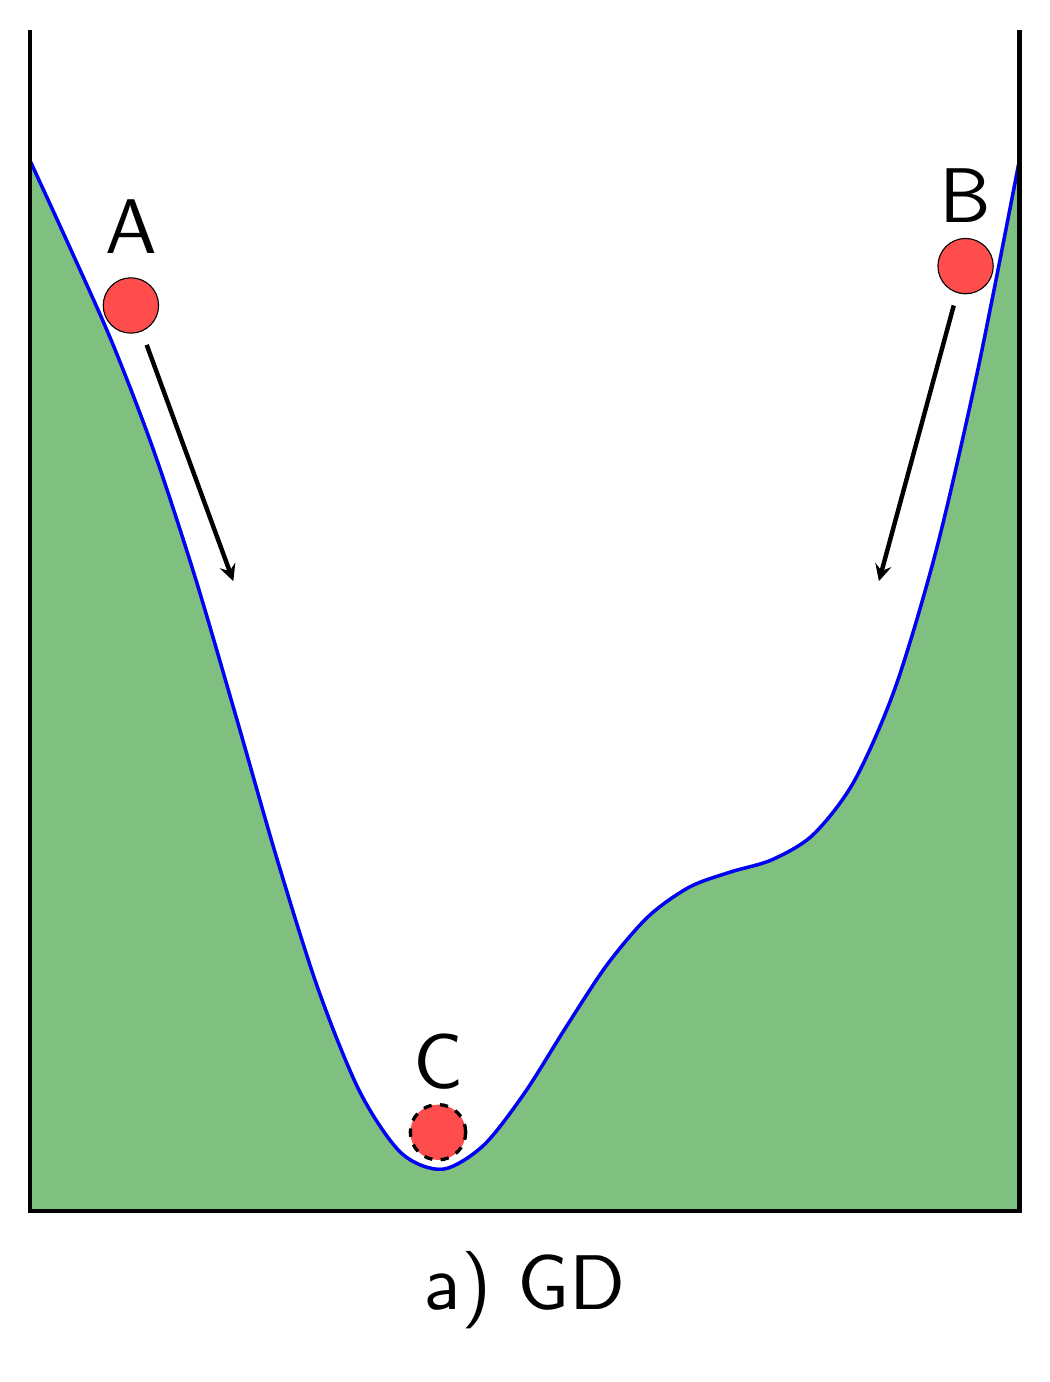
\begin{tikzpicture}[>= stealth]
    \begin{scope}[yscale = .3]
        
    \fill[draw = black, very thick, fill=green!50!black, opacity = .5] (-2*pi, 0) -- (-2*pi, 4*pi*pi+5) -- plot [domain=-2*pi:2*pi, smooth] (\x,{ \x*\x + 5*sin(\x r) + 5}) -- (2*pi, 4*pi*pi + 5) -- (2*pi, 0) -- cycle;
    \draw [very thick, blue] plot[ domain=-2*pi:2*pi, smooth] (\x,{\x*\x + 5 + 5*sin(\x r)});
    \draw [black, ultra thick ](-2*pi, 50) -- (-2*pi, 0) -- (2*pi, 0) -- (2*pi, 50);

    \end{scope}
    \draw [fill = red!70, draw = black] (-5, 11.5) circle (10pt);
    \node [scale = 2.8] at (-5, 12.5) {A};
    \draw [ultra thick, ->] (-4.8, 11) -- (-3.7, 8);

    \draw [fill = red!70, draw = black] (5.6, 12) circle (10pt);
    \node [scale = 2.8] at (5.6, 12.9) {B};
    \draw [ultra thick, ->] (5.45, 11.5) -- (4.5, 8);
    \draw [dashed, very thick, fill = red!70, draw = black] (-1.1, 1) circle (10pt);
    \node [scale = 2.8] at (-1.1, 1.9) {C};
    \node [scale = 2.8] at (0, -1) {a) GD};
\end{tikzpicture}
~~~~
% block B 
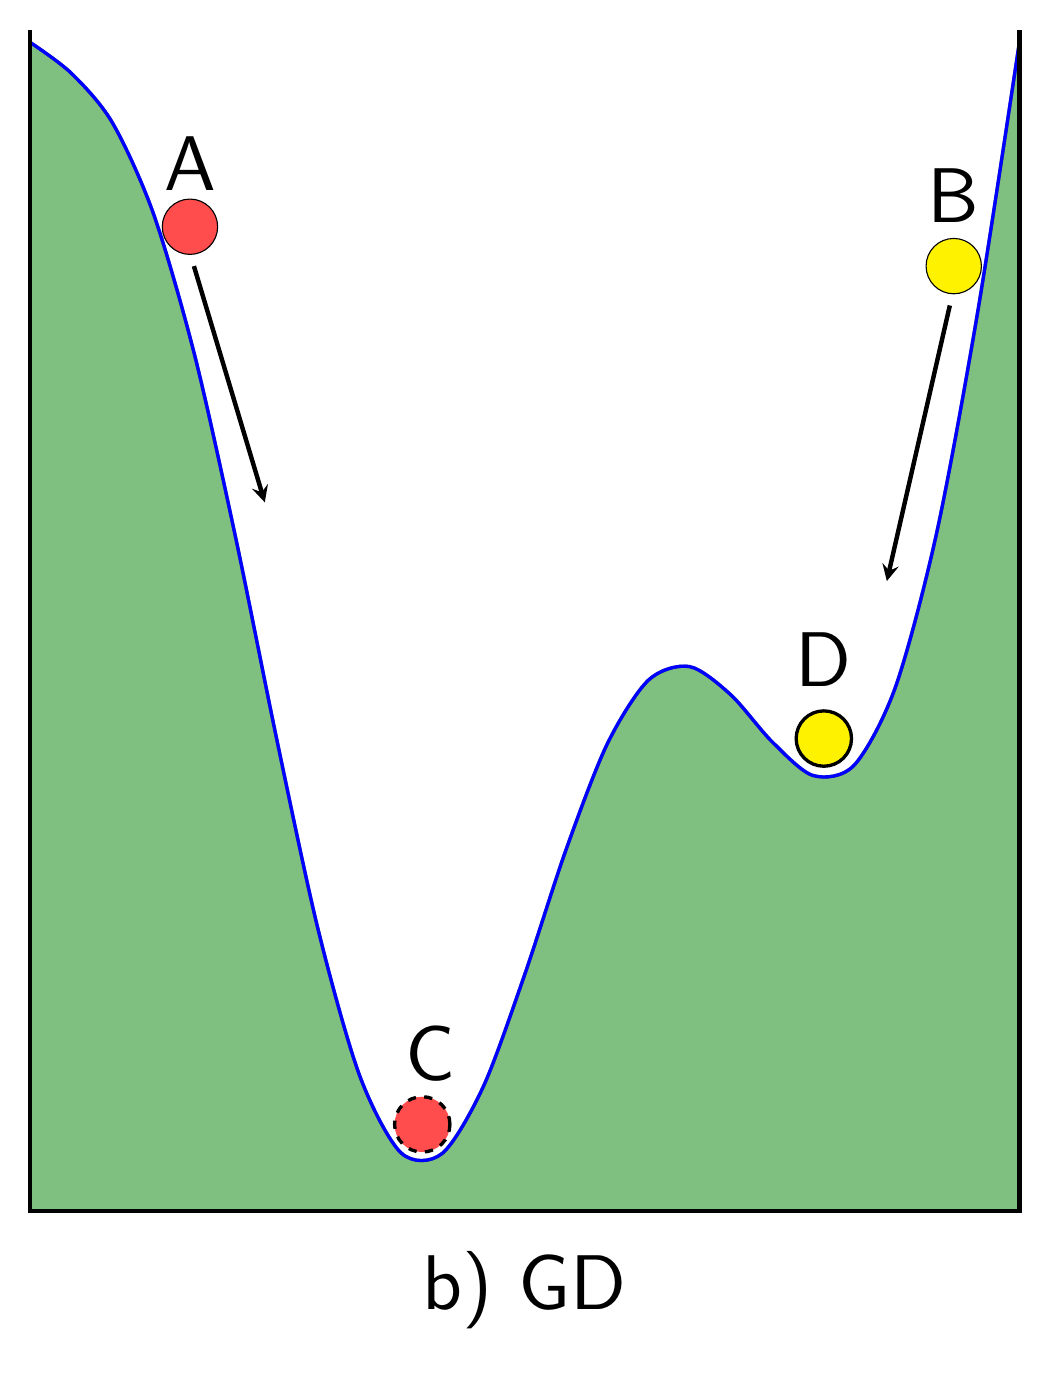
\begin{tikzpicture}[>= stealth]
    \begin{scope}[yscale = .3]
        
    \fill[draw = black, very thick, fill=green!50!black, opacity = .5] (-2*pi, 0) -- (-2*pi, 4*pi*pi+5) -- plot [domain=-2*pi:2*pi, smooth] (\x,{ \x*\x + 10*sin(\x r) + 10}) -- (2*pi, 4*pi*pi + 10) -- (2*pi, 0) -- cycle;
    \draw [very thick, blue] plot[ domain=-2*pi:2*pi, smooth] (\x,{\x*\x + 10 + 10*sin(\x r)});
    \draw [black, ultra thick ](-2*pi, 50) -- (-2*pi, 0) -- (2*pi, 0) -- (2*pi, 50);

    \end{scope}
    \node [scale = 2.8] at (-4.25, 13.3) {A};
    \draw [fill = red!70, draw = black] (-4.25, 12.5) circle (10pt);
    \draw [ultra thick, ->] (-4.2, 12) -- (-3.3, 9);

    \draw [dashed, very thick, fill = red!70, draw = black] (-1.3, 1.1) circle (10pt);
    \node [scale = 2.8] at (-1.2, 2) {C};

    %%%%%%%%%%%%%%%%%%%%
    \draw [fill = yellow!100!black, draw = black] (5.45, 12) circle (10pt);
    \node [scale = 2.8] at (5.45, 12.9) {B};
    \draw [ultra thick, ->] (5.4, 11.5) -- (4.6, 8);
    \draw [very thick, fill = yellow!100!black, draw = black] (3.8, 6) circle (10pt);
    \node [scale = 2.8] at (3.8, 7) {D};

    \node [scale = 2.8] at (0, -1) {b) GD};
\end{tikzpicture}
~~~~
% block C
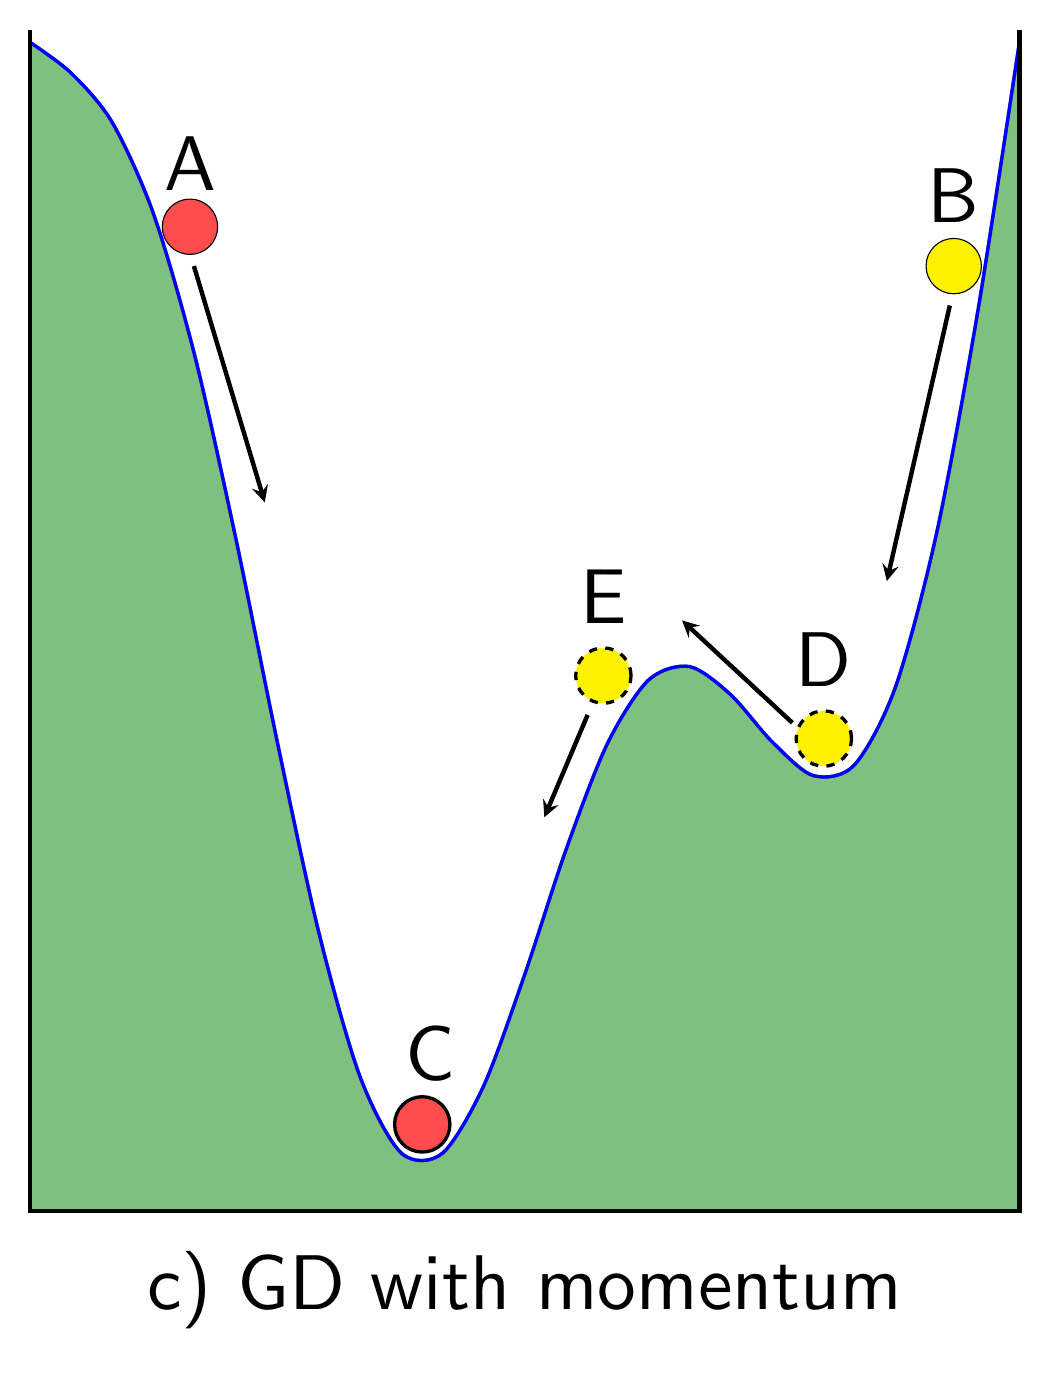
\begin{tikzpicture}[>= stealth]
    \begin{scope}[yscale = .3]
        
    \fill[draw = black, very thick, fill=green!50!black, opacity = .5] (-2*pi, 0) -- (-2*pi, 4*pi*pi+5) -- plot [domain=-2*pi:2*pi, smooth] (\x,{ \x*\x + 10*sin(\x r) + 10}) -- (2*pi, 4*pi*pi + 10) -- (2*pi, 0) -- cycle;
    \draw [very thick, blue] plot[ domain=-2*pi:2*pi, smooth] (\x,{\x*\x + 10 + 10*sin(\x r)});
    \draw [black, ultra thick ](-2*pi, 50) -- (-2*pi, 0) -- (2*pi, 0) -- (2*pi, 50);

    \end{scope}
    \node [scale = 2.8] at (-4.25, 13.3) {A};
    \draw [fill = red!70, draw = black] (-4.25, 12.5) circle (10pt);
    \draw [ultra thick, ->] (-4.2, 12) -- (-3.3, 9);

    \draw [very thick, fill = red!70, draw = black] (-1.3, 1.1) circle (10pt);
    \node [scale = 2.8] at (-1.2, 2) {C};

    %%%%%%%%%%%%%%%%%%%%
    \draw [fill = yellow!100!black, draw = black] (5.45, 12) circle (10pt);
    \node [scale = 2.8] at (5.45, 12.9) {B};
    \draw [ultra thick, ->] (5.4, 11.5) -- (4.6, 8);
    \draw [dashed, very thick, fill = yellow!100!black, draw = black] (3.8, 6) circle (10pt);
    \node [scale = 2.8] at (3.8, 7) {D};

    \draw [ultra thick, ->] (3.4, 6.2) -- (2, 7.5);
    \draw [dashed, very thick, fill = yellow!100!black, draw = black] (1, 6.8) circle (10pt);
    \node [scale =2.8] at (1, 7.8) {E};
    \draw [ultra thick, ->] (0.8, 6.3) -- (0.25, 5);
    % \draw [->] 

    \node [scale = 2.8] at (0, -1) {c) GD with momentum};
\end{tikzpicture}
\end{document}
